\documentclass[a4paper]{article}
%\usepackage{simplemargins}

\usepackage[
	pdftitle={The KonGeoS Network - Working Groups and Outreach},
	pdfsubject={The KonGeoS Network - Working Groups and Outreach},
	pdfauthor={Florian Thiery, Julius Fintzen},
	pdfkeywords={KonGeoS}
]{hyperref}

\input{doiCmd}
%\RequirePackage{doi}
%\usepackage[square]{natbib}
\usepackage{amsmath}
\usepackage{amsfonts}
\usepackage{amssymb}
\usepackage{graphicx}

\begin{document}
\pagenumbering{gobble}

\Large
 \begin{center}
The KonGeoS Network -\\ Working Groups and Outreach\\ 

\hspace{10pt}

% Author names and affiliations
\large
Florian Thiery$^1$, Julius Fintzen$^2$\\

\hspace{10pt}

\small  
$^1$$^,$$^2$ Konferenz der Geod{\"a}sieStudierenden\\
$^1$ thiery@kongeos.de, $^2$ fintzen@kongeos.de\\

\end{center}

\normalsize

The Konferenz der Geod{\"a}sieStudierenden (KonGeoS, engl. \textit{conference of geodesy students}) is a student network and student association for more than 1000 geodesy students in the German speaking countries: Germany, Austria and Switzerland. Today, KonGeoS consists of 22 university members, 18 from Germany, 2 from Austria and 2 from Switzerland, cf. Fig.~\ref{Abb1}. In Germany, two types of universities are existing: traditional `universities` (e.g. University, TU, ...) and the applied `universities` (formally Fachhochschule, FH). In 2012, the two organisations `ARGEOS` (Uni) and `KonVerS` (FH) joint together regarding to the Bologna process. The KonGeoS members build a huge network which is supported by the `KonGeoS supporting association` (dt. \textit{F{\"o}rderverein der Konferenz der Geod{\"a}siestudierenden e.V.}, FV KonGeoS e.V.). These organisations are embedded into a `professional association framework` of the German speaking countries.

\begin{figure}[!h]
\begin{center}
\includegraphics[height=10cm]{karte.png}
\caption{KonGeoS members (CC BY 4.0 KonGeoS)}
\label{Abb1}
\end{center}
\end{figure}

KonGeoS is directly connected with the DVW - Society for Geodesy, Geoinformation and Land Management e.V. and the VDV (Association of German Surveying Engineers). KonGeoS own seats in the DVW Working Group 1 `Profession/Education` as well as in the federal board of the VDV. KonGeoS is also in contact with other German professional associations, as well as from Austria and Switzerland, cf. Fig.~\ref{Abb2}.

\begin{figure}[!h]
\begin{center}
\includegraphics[width=10cm]{VerbandsUebersichtDeutschland.png}
\caption{KonGeoS and the Professional Associations of German speaking countries (CC BY 4.0 KonGeoS, Stefan Thoben, Florian Thiery)}
\label{Abb2}
\end{center}
\end{figure}

In an international context, KonGeoS cooperates with the `International Geodetic Student Organization` (IGSO) which organises the `International Geodetic Student Meeting` (IGSM). There is also a cooperation between the FIG (International Federation of Surveyors) and the `FIG Young Surveyors` Network, cf. Fig.~\ref{Abb3}.

\begin{figure}[!h]
\begin{center}
\includegraphics[width=11cm]{GeodaetischesNetzwerk.png}
\caption{KonGeoS and the international Professional Associations (CC BY 4.0 KonGeoS, Stefan Thoben, Florian Thiery)}
\label{Abb3}
\end{center}
\end{figure}

The network character of KonGeoS is kept in several working groups, where the students and alumni are discussing and create documents for publishing. The current working groups are: `young surveyors and junior support` (Nachwuchs, YS), `public relations and web` ({\"O}ffentlichkeitsarbeit), `associations` (Vereine- und Verb{\"a}nde, A), `studies` (Studium, S), `project` (Projekt) and `dinosaurs` (Saurier). The `WG-A` has to maintain contact to the various mentioned professional associations which supports KonGeoS. The `WG-S` is discussing on possible improvements for the general studying experience and maintains the `Master vermisst` (engl. master missed) list, which lists possible geodesy master study programs at German speaking universities and is downloadable on the KonGeoS website. The `WG-YS` do a evaluation of freshmen survey sheets, publish the results and discuss new ideas on geodesy recruitment campaigns. The results of the survey sheets are downloadable on the web. Below some of the results for 2019 are listed, based on 325 freshmen of 15 universities.

\begin{figure}[!h]
\begin{center}
\includegraphics[width=12cm]{wg-ys1.png}
\caption{gender distribution (freshmen survey 2019) (CC BY 4.0 KonGeoS, Wilfried Jansky, Florian Thiery)}
\label{Abb4}
\end{center}
\end{figure}

The survey shows (cf. Fig.~\ref{Abb4}), that nearly 75\% of the geodesy freshmen are male, only ca. 25\% are female. This ratio have to be adjusted in the future! In case of the motivations to start studying the a specific university, we cannot see a primary reason, the closeness to the home town, the university reputation and subjects, the city itself, family relations as well as the option for a master study is nearly equally important, cf. Fig.~\ref{Abb5}. Most of the surveying student want to work in the `classical` surveying sector: Fig.~\ref{Abb6} shows that more than 35\% of all participants want to work in the surveying administration, an engineering office or as {\"O}bVI, an administrational engineer. Only ~20\% want to work in the industry and ~12\% in software companies. One eighth may work in research and the university after their studies. Fig.~\ref{Abb7} shows that nearly half of the freshman want to work into `surveying`, only one quarter into the IT related fields.

\begin{figure}[!ht]
\begin{center}
\includegraphics[width=12cm]{wg-ys2.png}
\caption{why did you study where you study? (freshmen survey 2019) (CC BY 4.0 KonGeoS, Wilfried Jansky, Florian Thiery)}
\label{Abb5}
\end{center}
\end{figure}

\begin{figure}[!ht]
\begin{center}
\includegraphics[width=12cm]{wg-ys3.png}
\caption{future working area? (freshmen survey 2019) (CC BY 4.0 KonGeoS, Wilfried Jansky, Florian Thiery)}
\label{Abb6}
\end{center}
\end{figure}

\begin{figure}[!ht]
\begin{center}
\includegraphics[width=12cm]{wg-ys4.png}
\caption{future working field? (freshmen survey 2019) (CC BY 4.0 KonGeoS, Wilfried Jansky, Florian Thiery)}
\label{Abb7}
\end{center}
\end{figure}

\begin{figure}[!ht]
\begin{center}
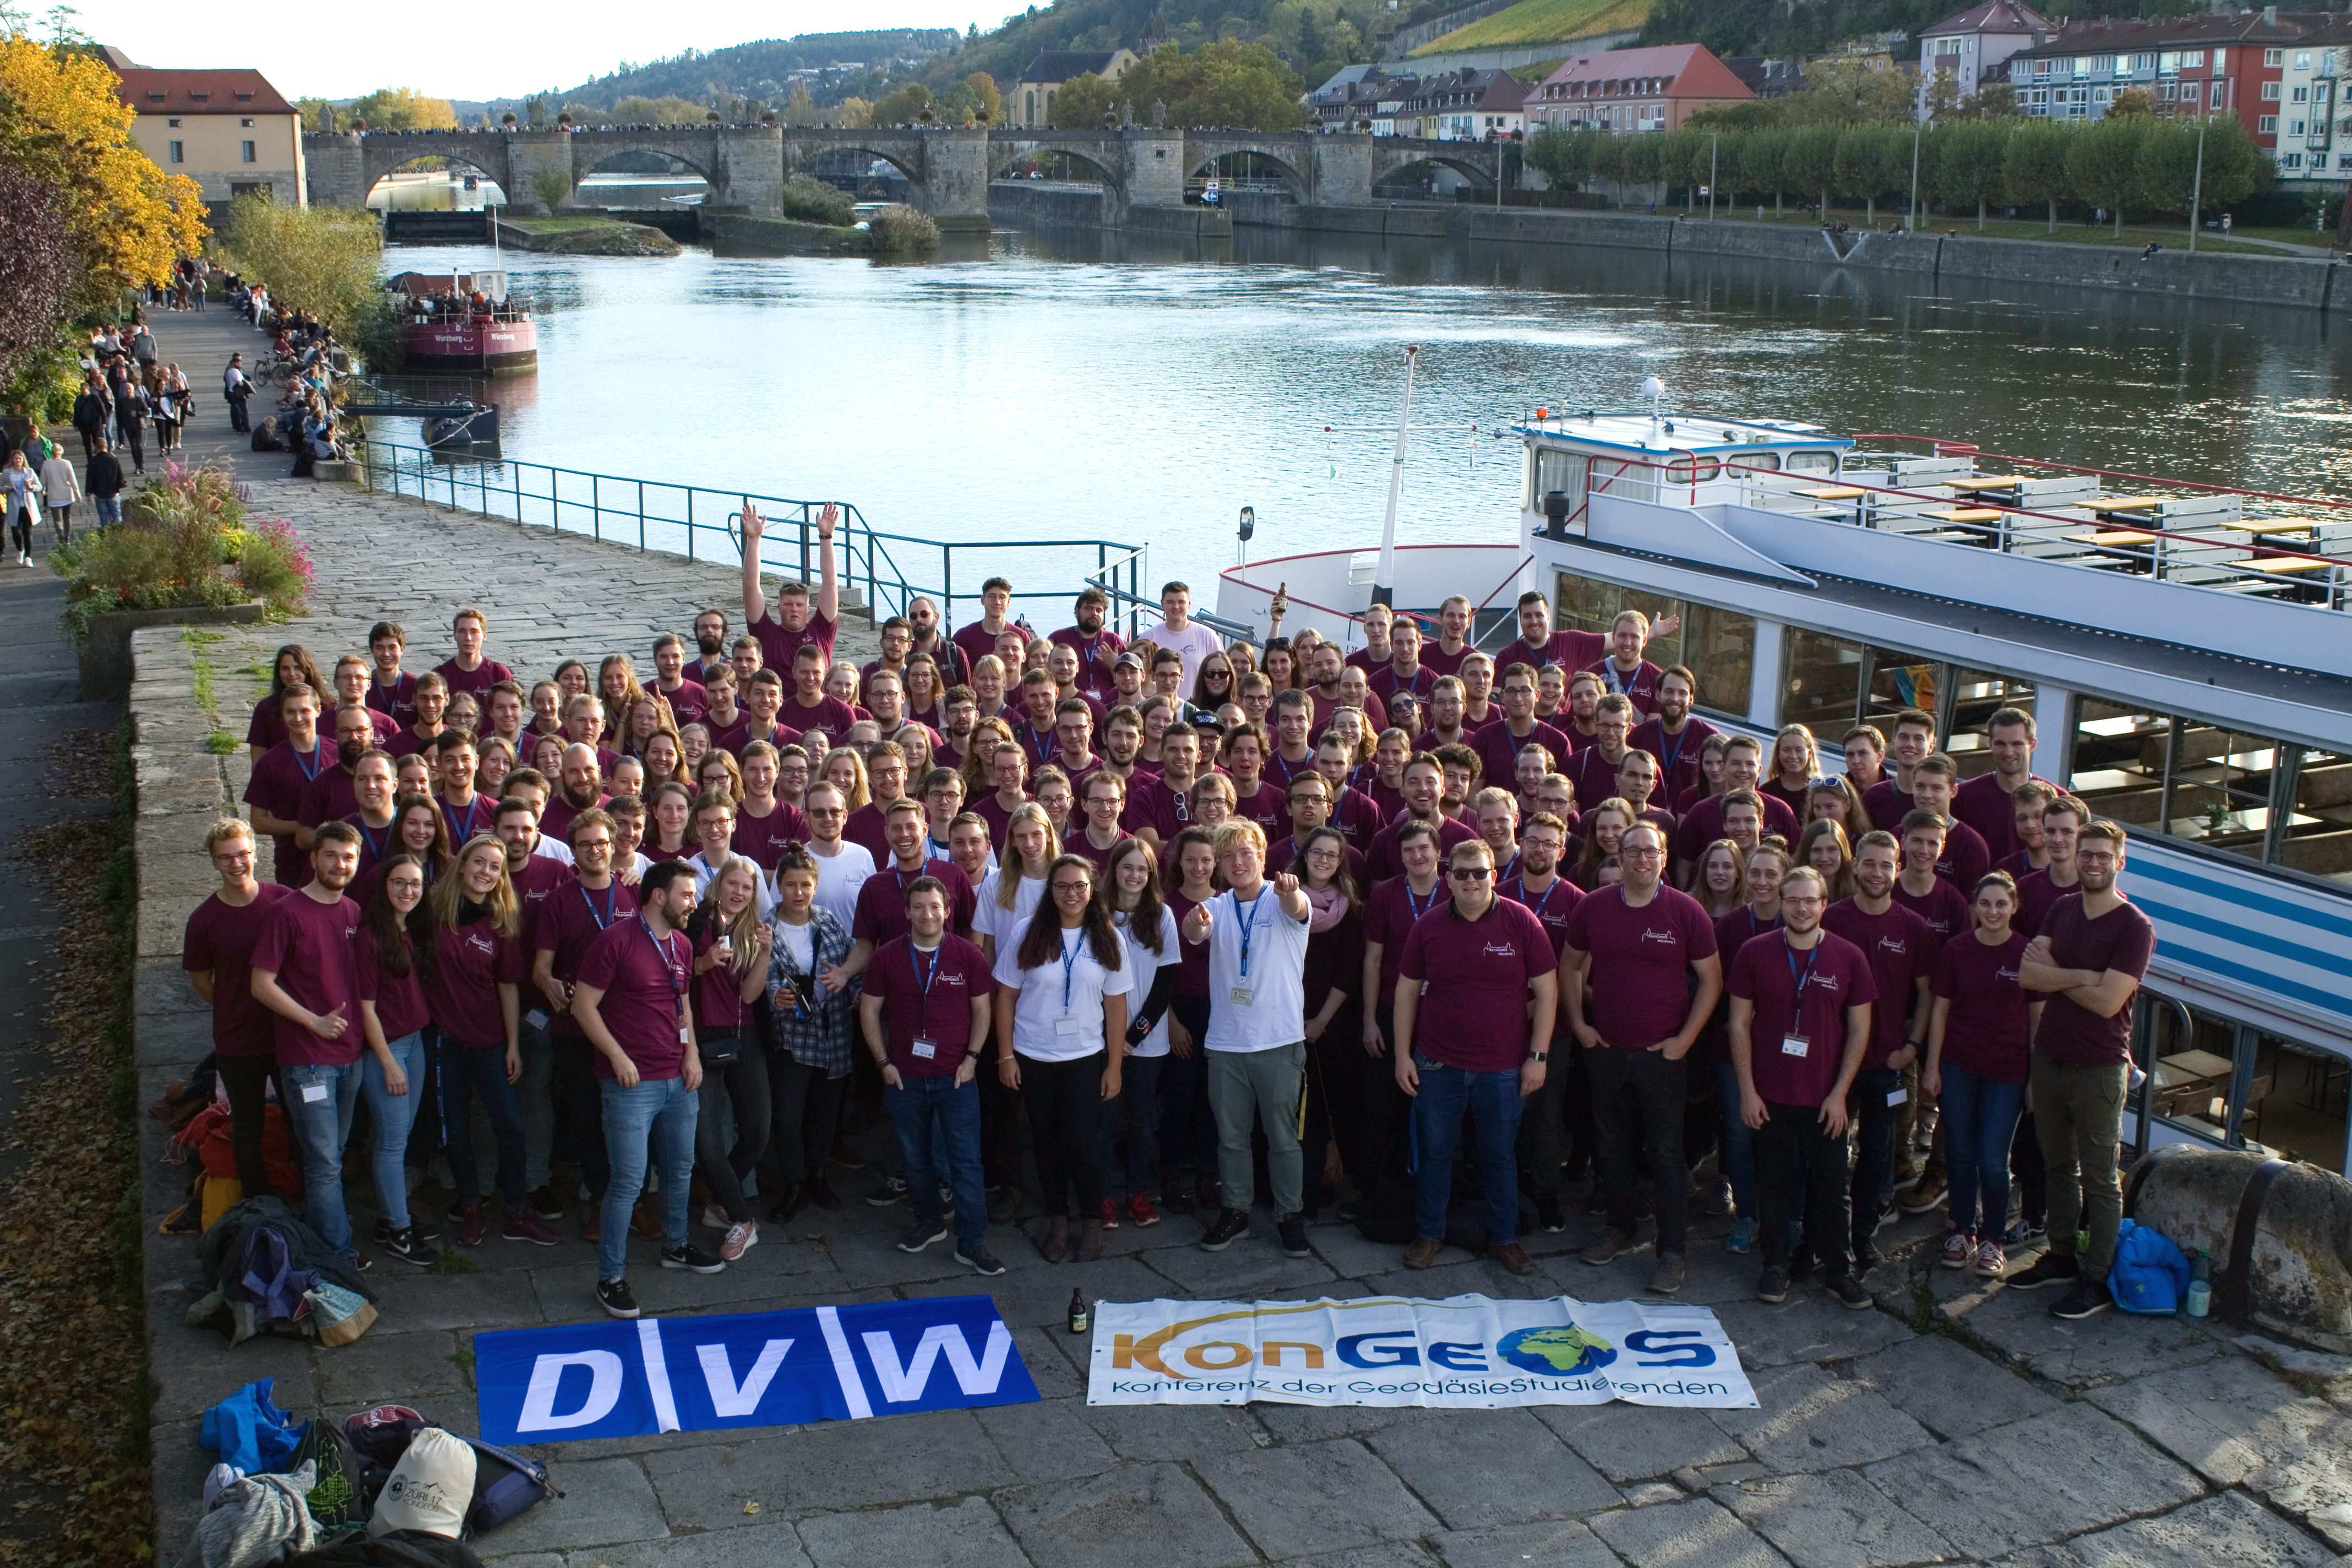
\includegraphics[width=12cm]{IMG_7435_01.jpg}
\caption{KonGeoS Wuerzburg 2019 (CC BY 4.0 KonGeoS Wuerzburg)}
\label{Abb8}
\end{center}
\end{figure}

\end{document}